\section{Zielsetzung}
\label{sec:Ziel}
In diesem Versuch sollen freie Elektronen aus einer Metaloberfläche erzeugt werden. Dazu wird der Effekt der thermischen Elektronenemission verwendet. Es wird die 
Temperaturabhängigkeit dieses Effektes untersucht. 

\section{Theorie}
\label{sec:Theorie}
Bei der thermischen Elektronenemission sollen Elektronen durch Erhitzung eines Materials aus diesem befreit werden. Dies gestaltet sich für die meisten Materialien 
schwierig, da die Elektronen meist sehr stark an die Atome gebunden sind. Daher kann ein Elektronen, trotz der zugeführten kinetischen Energie häfig nicht austreten. 
Erst wenn bestimmte Materialien in einen Plasmazustand übergehen, können freie Elektronen leichter erzeugt werden. Da dies nicht effizient ist, wird stattdessen eine Eigenschaft
von Metallen verwendet, welche es ermöglicht thermische Elektronenemission schon unter vereinfachten Bedingungen zu erreichen. Dabei handelt es sich um die elektrische 
Leitfähigkeit von Metallen. Metalle besitzen eine hohe Leitfähigkeit, da sie \textit{Leitungselektronen} besitzen. Diese \textit{Leitungselektronen} sind nicht fest an 
Atome gebunden, sonder können sich fast vollkommen frei in dem Metall bewegen. Intrinsisch entsteht so ein inneres periodisches Gitter aus Kationen, welches von einer äußeren
Hülle aus \textit{Leitungselektronen} umflossen wird. 
In dem Material bildet sich ein annähernd konstantes Potential. Außerhalb des Metalls ist das Potential aber veschwindet gering. Die Elektronen befinden sich daher in einer Art
\textit{Potentialtopf}. Elektronen mit genügend Energie können diesen \textit{Potentialtopf} verlassen. Diese Elektronen sind dann freie Elektronen. Allerdings entstehen diese 
nur, wenn die Elektronen im \textit{Potentialtopf} die benötigte \textit{Austrittsarbeit} leisten.
Der hypothetische \textit{Potentialtopf}, in dem sich die Elektronen aufhalten ist in \autoref{fig:Potentialtopf} dargestellt.
\begin{figure}
    \centering
    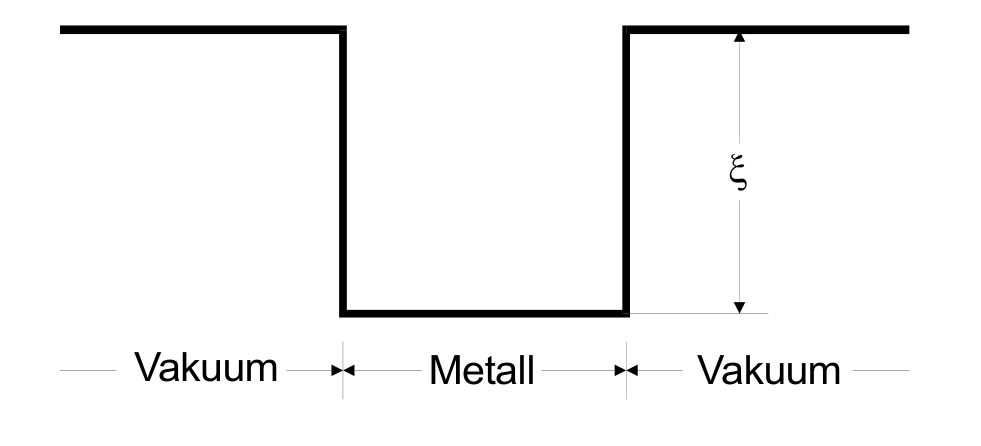
\includegraphics[width = 0.5\textwidth]{content/Potentialtopf.png}
    \caption{Potentialtopfmodell des Elektrons im Metall \cite{v504}.}
    \label{fig:Potentialtopf}
\end{figure}

\subsection{Austrittsarbeit und Energieverteilung der Leitungselektronen}
\label{subsec:Austrittsarbeit}
Die Austrittsarbeit der Elektronen wird nun quantenmechanisch betrachtet. Elektronen haben diskrete voneinander veschiedene Energieniveaus. Zusätzlich haben Elektronen 
den Spin $s = \pm\frac{1}{2}$, weshalb sie dem \textit{Pauli-Verbot} unterliegen. Dieses besagt, dass ein diskreter Energiezustand höchstens von zwei Elektronen mit 
unterschiedlichem Spin besetzt werden kann. Aus diesen Eigenschaften von Elektronen folgt, dass sie auch bei $\qty{0}{\kelvin}$ eine endliche Energie bestitzen. Diese Energie
wird \textit{Fermische Grenzenergie} $\xi$ genannt. Die Wahrscheinlichkeit, dass sich ein Elektron in einem bestimmten Energiezustand befindet ist gegeben durch die
\textit{Fermi-Diracsche Verteilungsfunktion}. Für kleine Temperaturen ist diese Verteilungsfunktion durch
\begin{equation}
    f(E) \approx e^\frac{\xi - E}{kT}
\end{equation}
gegeben.

\subsection{Die Hochvakuum-Diode}
\label{subsec:Hochvakuum-Diode}
Thermische Elektronenemission kann auch unter normalen Bedingungen stattfinden, allerdings ist der Nachweis dieses Effektes nur mit angepassten Umgebungsbedingungen möglich.
Diese Bedingungen birgt die \textit{Hochvakuum-Diode}. Das Vakuum ist nötigt, da die frei werdenden Elektron sonst mit den Luftmolekülen wechselwirken und somit nicht gemessen
werden könnten. Außerdem liegt eine Spannung zwischem dem Material, aus welchem die Elektronen austreten, und einer Kathode an. Durch dieses elektrische Feld erfahren die 
Elektron eine Beschleunigung. Dabei entsteht durch die endliche Geschwindigkeit der Elektronen eine Raumladungsdichte, welche in \autoref{subsec:Raumladungsgebiet} beschrieben
wird. In einer Hochvakuum-Diode werden die Elektronen durch den \textit{Glühelektrischen Effekt} aus einem Draht ausgelöst. Eine Skizze einer Hochvakuum-Diode ist in 
\autoref{fig:Vakuumdiode} dargestellt.

\begin{figure}
    \centering
    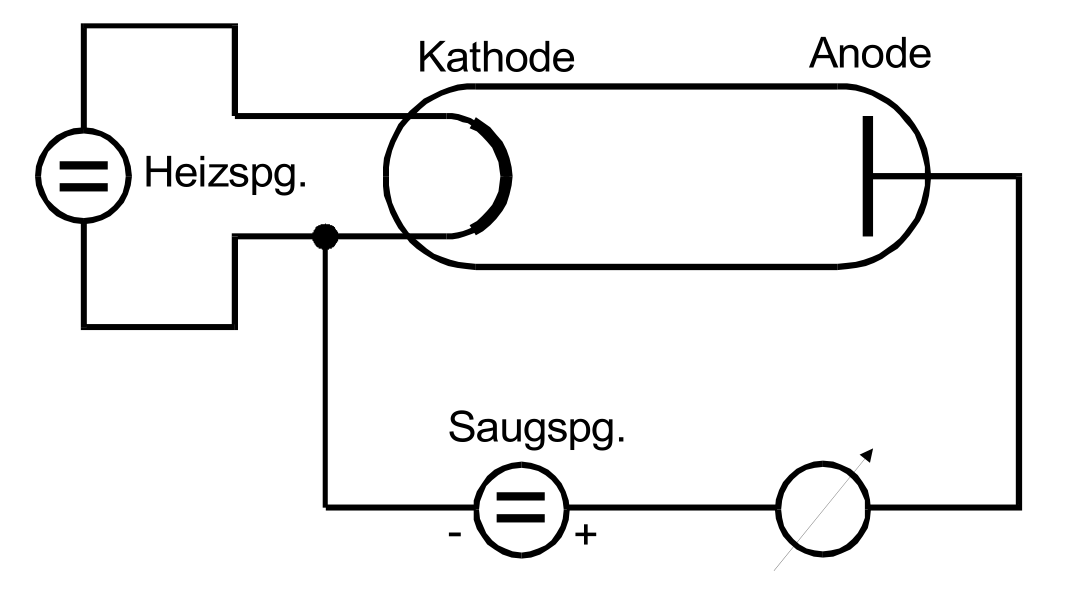
\includegraphics[width = .5\textwidth]{content/Vakuumdiode.png}
    \caption{In dieser Abbildung ist der schematische Aufbau einer Hochvakuumdiode dargestellt.\cite{v504}.}
    \label{fig:Vakuumdiode}
\end{figure}

\subsection{Das Raumladungsgebiet}
\label{subsec:Raumladungsgebiet}
Freie Elektronen, welche sich zwischen Kathode und Anode befinden, erzeugen eine Raumladungsdichte, welche der Kontinuitätsgleichung genügen muss. Da die Raumladungsdichte 
eine Funktion des Ortes ist, kann sie nicht homogen sein. Daher kann bei geringer Elektronenzahl das elektrische Feld zwischen Kathode und Anode abgeschirmt werden und es 
können somit nicht alle elektronen die Kathode erreichen. Daher sinkt der Kathodenstrom, welcher dann durch 
\begin{equation}
    \label{eqn:langmuirraumladung}
    j = \frac{4}{9}\epsilon_0\sqrt{\frac{2eV^3}{m_0a^4}}
\end{equation}
beschrieben wird.

\subsection{Kennlinie einer Hochvakuum-Diode}
\label{subsec:Kennlinie}
Die Kennlinie einer Hochvakuum-Diode ist gegeben durch den gemessenen Strom in Abhängigkeit zur Beschleunigungsspannung. Diese Kennlinie kann in drei Bereiche unterteilt werden.
Diese drei Bereiche werden in \autoref{fig:Kennlinie} dargestellt. Die Phsyik des Raumladungsgebietes wurde bereits in \autoref{subsec:Raumladungsgebiet} beschrieben.
Die verbleibende zwei Gebiete werden in den nächsten beiden Abschnitten diskutiert.

\begin{figure}
    \centering
    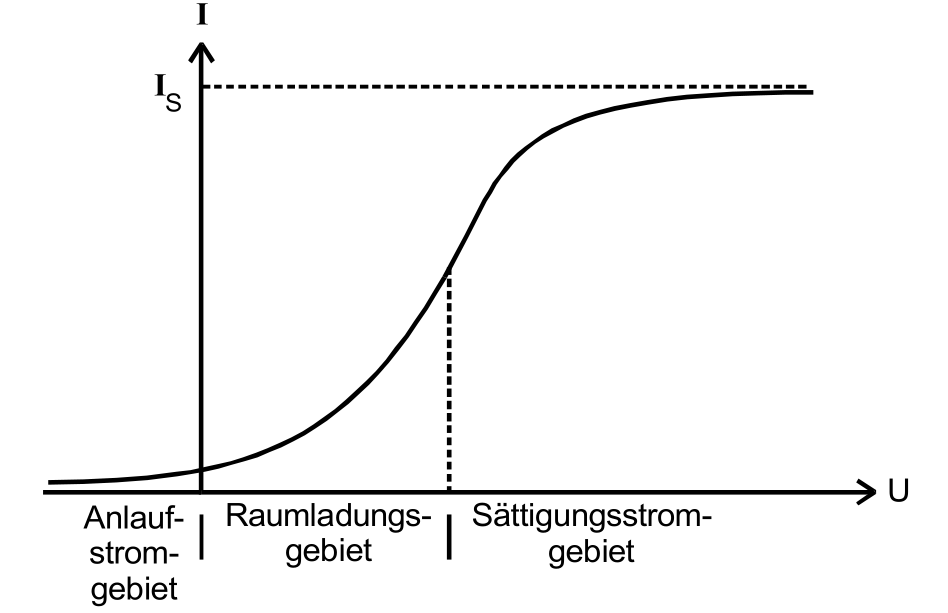
\includegraphics[width = .5\textwidth]{content/Kennlinie.png}
    \caption{Kennlinie einer Hochvakuumdiode und Unterteilung in wichtige Bereiche des Stroms \cite{v504}.}
    \label{fig:Kennlinie}
\end{figure}

\subsection{Das Anlaufstromgebiet}
\label{subsec:Anlaufstromgebiet}
Das Anlaufstromgebiet beschreibt einen Spannungsbereich von $U \leq 0$. Hier ist die intuitive Erwartung, dass kein Strom gemessen werden kann. Allerdings fällt experimentell
auf, dass ein kleiner Strom gemessen werden kann. Dieser existiert, da die ausgelösten Elektronen nicht ohne resultierende kinetische Energie ausgelößt werden können. Diejenigen
Elektron mit genug kinetischer Energie können gegen kleine Gegenfelder dennoch zur Kathode gelangen und somit einen Strom erzeugen. Dieser Strom folgt einer 
Beschreibung durch
\begin{equation}
    \label{eqn:Anlaufstromgebiet}
    j_{\text{Anlauf}}(V) = j_0 \symup{e}^{\left(-\frac{e\Phi_0 + eV}{kT}\right)} = \text{const}\symup{e}^{\left(-\frac{e_0V}{kT}\right)}
\end{equation}
mit der Temperatur $T$ und dem Potential $V$.

\subsection{Sättigungsstromgebiet}
\label{subsec:Sättigungsstromgebiet}
Im Sättigungsstromgebiet läuft der gemessene Strom gegen einen Grenzwert. Dieser konstante Strom wird Sättigungsstrom $I_s$ genannt. Dieser ist gegeben durch die Gleichung
\begin{equation}
    \label{eqn:Sättigungsstrom}
    I_s(T,f) = f j_s = 4\pi\frac{em_0k^2}{h^3}T^2\symup{e}^{\left(-\frac{e\Phi}{kT}\right)},
\end{equation}
wobei $j_s$ die sogenannte \textit{Richardson-Gleichung} ist. Die \textit{Richardson-Gleichung} betrachtet wie viele Elektronen mindestens die nötige Austrittsenergie besitzen, 
damit der maximale Strom beschrieben werden kann. In der Gleichung \ref{eqn:Sättigungsstrom} beschreibt $f$ die Kathodenoberfläche.

\subsection{Abschätzung der Temperatur der Kathode}
\label{subsec:Temperatur}
Die Temperatur der Diode steht in direkter Abhängigkeit zur Strahlungsleistung $N_{\text{WL}}$. Diese ist nach dem \textit{Stefan-Bolzmann-Gesetz} gegeben durch
\begin{equation*}
    N_{\text{Str}} = f\mu\sigma T^4 ,
\end{equation*}
wobei $\sigma = \qty{5.7}{\pico\watt\per\centi\metre\squared\kelvin^4}$ und $\eta$ der Emissionsgrad der Kathode ist.
Aus dem Energiesatz folgt nun für die Leistungsbilanz mit der zugeführten Leistung $N_{zu} = UI$
\begin{equation}
    \label{eqn:Temp}
    UI = f\mu\sigma T^4 + N_{\text{WL}} ,
\end{equation}
wobei $N_{\text{WL}}$ die Wärmeleistung der Kathode ist. Aus der Gleichung \ref{eqn:Temp} kann nun die Temperatur der Kathode abgeschätzt werden.